\documentclass[a4paper,11pt]{article}
\usepackage[margin=3.3cm]{geometry}
\linespread{1}
\usepackage[T1]{fontenc}
\usepackage[utf8]{inputenc}
\usepackage{tikz}
\usepackage{array}
\usepackage{amsmath}
\usepackage{float}
\newcommand{\resetfont}{\renewcommand{\familydefault}{lmtt}\normalfont}
\renewcommand{\contentsname}{TABLE OF CONTENTS}
\frenchspacing
\begin{document}
\pagenumbering{gobble}
\resetfont
\title{\vspace{-1cm} \Huge UBERPUTER ATM PROTOCOL SPECIFICATION DRAFT REV.1}
\author{Mikael Forsberg <miforsb@kth.se>\\ Robin Gunning <rgunning@kth.se>\\ $\quad$\\ \small Programmeringsparadigm DD1361\\ \small Kungliga Tekniska Högskolan HT15}
\date{December 4, 1985}
\maketitle
\vfill \small
N.B: Radiometric dating indicates that this document is actually from 2015.
\newpage
$\quad$

\newpage
\tableofcontents
\newpage
\pagenumbering{arabic}
\section{INTRODUCTION}
\section{PROTOCOL}
\subsection{OVERVIEW}
\hfill\begin{minipage}{\dimexpr\textwidth-1.13cm}
The protocol consists of three major components: a language dataset,
a set of message packets, and rules for the flow and ordering of messages.
The language dataset contains all strings needed for a client user
interface. The set of message packets contains all messages required
to be supported by servers and clients. Finally, compliant servers and
clients are required to follow all rules for flow and message ordering.

\vspace{0.3cm}

The language dataset is not constant, and clients are not supposed
to define or implement a copy of it themselves. Instead, clients should
retrieve the dataset from the server, and should also periodically check
for updates to the dataset. Both of these actions are performed by
sending a message of type UPDATE REQUEST (section \ref{client_update_req}
on page \pageref{client_update_req}). Clients should, however, keep
a cached copy of the dataset in order to avoid superfluous network
traffic.

\vspace{0.3cm}

The message packets and flow rules are centered on the basic principle
of clients receiving one or more MENU ITEMs containing instructions
for sending back ACTIONs. These exchanges cover nearly all of the
functionality of a session. The only predefined messages a client should
implement are UPDATE REQUEST, MENU REQUEST and ACTION. All other
expected functionality such as authentication will be determined at
runtime by MENU ITEMs sent from a server.

\vspace{0.3cm}
An ACTION can contain instructions for a client to send and / or
receive a single 32-bit integer value, and can also contain an
instruction for a client to receive an immediate follow-up action
that a client should execute directly. This principle of follow-up
actions is used to chain actions together, facilitating exchanges
of several values in sequence.

\end{minipage}
\newpage

\subsection{LANGUAGE DATASET: FORMAT}
\hfill\begin{minipage}{\dimexpr\textwidth-1.3cm}
The language dataset is supplied in a YAML-compatible format defined
by the following grammar, with starting nonterminal <Data>:

\begin{verbatim}
<Data> ::= <Pair> | <List> | <Pair> CR <Data> | <List> CR <Data>
<Pair> ::= <Value> : <Value>
<Value> ::= [A-Za-z0-9_]+ | ' [A-Za-z0-9_]+ ' | " [A-Za-z0-9_]+ "
<List> ::= <Value> : CR <ListValues>
<ListValues> ::= <Indent> <Pair> | <Indent> <Pair> CR <ListValues>
<Indent> ::= SPACE SPACE SPACE
\end{verbatim}
\end{minipage}
\vspace{0.5cm}

\subsection{LANGUAGE DATASET: EXAMPLE}
\label{lang_example}
\hfill\begin{minipage}{\dimexpr\textwidth-1.13cm}
The following is an example language dataset.

\rule{11cm}{0.7pt}
\begin{verbatim}
_Version: 2015120408
_Useful:
   change_language : 16
   press_any_key_to_continue : 17
English:
   0: ""
   1: "Welcome to UBERBANK"
   2: Balance
   3: Deposit
   4: Withdraw
   16: Change language
   17: Press any key to continue
Svenska:
   0: ""
   1: "Välkommen till UBERBANK"
   2: Saldo
   3: Insättning
   4: Uttag
   16: Byt språk
   17: Tryck valfri tangent för att fortsätta
\end{verbatim}
\rule{11cm}{0.7pt}
\end{minipage}
\vspace{0.5cm}

\subsection{LANGUAGE DATASET: TRANSMISSION, UPDATING}
\hfill\begin{minipage}{\dimexpr\textwidth-1.13cm}
The language dataset is transmitted from server to client using
the message packet UPDATE (section \ref{server_update} on page \pageref{server_update}).
This packet is sent in response to a client request using the
UPDATE REQUEST (section \ref{client_update_req} on page \pageref{client_update_req}).
As part of the UPDATE REQUEST, a client should include the value
of the special field ''\_Version'' contained in the language dataset
(see example above), which is used by a server
to decide whether or not to send an update. If there is no
update available a server will not send the UPDATE message, but
will instead simply reply with an OK (section \ref{server_ok} on
page \pageref{server_ok}).

\end{minipage}
\newpage

\subsection{SYMBOLIC CONSTANTS}
\label{constants}
\hfill\begin{minipage}{\dimexpr\textwidth-1.13cm}
\begin{tabular}{l l}
SYMBOL & VALUE\\
\hline
MSG\_MENU\_REQUEST & 0\\
MSG\_MENU\_NUM\_ITEMS & 1\\
MSG\_ACTION & 2\\
MSG\_UPDATE\_REQUEST & 3\\
MSG\_MENU\_ITEM & 4\\
MSG\_OK & 5\\
MSG\_FAIL & 6\\
MSG\_UPDATE & 7\\
MSG\_RESPONSE & 8\\
 & \\
SYMBOL & VALUE\\
\hline
TYPE\_RECV\_FOLLOWUP & 32 \\
TYPE\_RECV\_UINT32 & 64 \\
TYPE\_SND\_UINT32 & 128 \\
\end{tabular}

\end{minipage}
\subsection{DATA FORMATS}
\hfill\begin{minipage}{\dimexpr\textwidth-1.2cm}
With the exception of the data field in the server-to-client
UPDATE message packet, all fields of all message packets contain
unsigned integers in network byte order (big-endian) of size
specified by the width of the field.
\end{minipage}

\subsection{MESSAGE PACKETS: CLIENT TO SERVER}
\subsubsection{UPDATE REQUEST}
\label{client_update_req}
\hfill\begin{minipage}{\dimexpr\textwidth-1.4cm}
To request an update from a server, a client should send the following
40-bit (5-byte) packet:

\vspace{0.2cm}

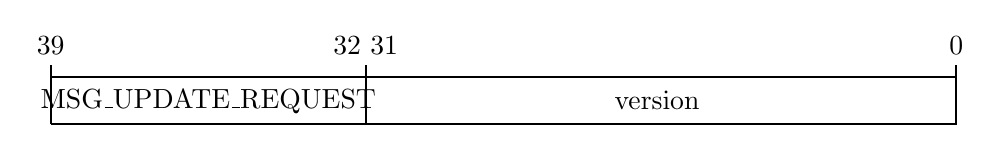
\begin{tikzpicture}
\draw[thick] (0,0) -- (11.5,0) -- (11.5,0.6) -- (0,0.6) -- (0,0);
\draw[thick] (0,0) -- (0,0.75) node[above] {39};
\draw[thick] (4,0) -- (4,0.75) node[above] {32 31};
\draw[thick] (11.5,0) -- (11.5,0.75) node[above] {0};
\draw[thick] (2,0) node[above] {MSG\_UPDATE\_REQUEST};
\draw[thick] (7.7,0.05) node[above] {version};
\end{tikzpicture}

\vspace{0.5cm}

The ''version'' field should contain the unsigned integer value contained
in the special field ''\_Version'' of the language dataset (see
section \ref{lang_example} on page \pageref{lang_example}). If
a client does not have any such value to send (e.g. before retrieving
the language dataset for the first time), the field should be set
to all zeroes (32-bit integer zero).

\vspace{0.3cm}

A server will reply in one of two ways. If there is an
update available, the reply will be an UPDATE
(section \ref{server_update} on page \pageref{server_update}).
Otherwise, the reply will simply be an OK
(section \ref{server_ok} on page \pageref{server_ok}).
\end{minipage}

\subsubsection{MENU REQUEST}
\label{menureq}
\hfill\begin{minipage}{\dimexpr\textwidth-1.4cm}
To request a list of available menu options, a client should send the
following 8-bit (1-byte) packet:

\vspace{0.2cm}

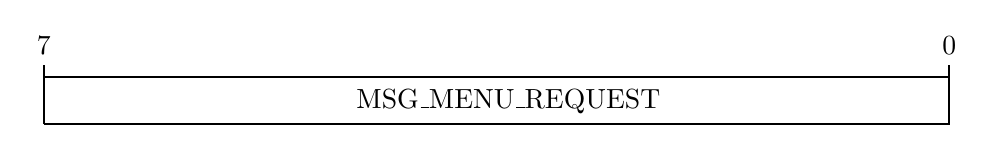
\begin{tikzpicture}
\draw[thick] (0,0) -- (11.5,0) -- (11.5,0.6) -- (0,0.6) -- (0,0);
\draw[thick] (0,0) -- (0,0.75) node[above] {7};
\draw[thick] (11.5,0) -- (11.5,0.75) node[above] {0};
\draw[thick] (5.9,0) node[above] {MSG\_MENU\_REQUEST};
\end{tikzpicture}

\vspace{0.5cm}

A server will reply with a single instance of MENU NUM ITEMS
(section \ref{server_menu_num_items} on page \pageref{server_menu_num_items})
containing the number N of menu items to follow, followed by
N instances of MENU ITEM
(section \ref{server_menu_item} on page \pageref{server_menu_item}).
\end{minipage}

\subsubsection{ACTION}
\label{action}
\hfill\begin{minipage}{\dimexpr\textwidth-1.4cm}
To perform an action, a client should send the following \\
64-bit (8-byte) packet:

\vspace{0.2cm}

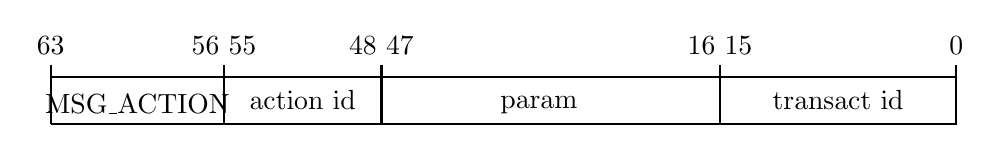
\begin{tikzpicture}
\draw[thick] (0,0) -- (11.5,0) -- (11.5,0.6) -- (0,0.6) -- (0,0);
\draw[thick] (0,0) -- (0,0.75) node[above] {63};
\draw[thick] (2.2,0) -- (2.2,0.75) node[above] {56 55};
\draw[thick] (4.2,0) -- (4.2,0.75) node[above] {48 47};
\draw[thick] (8.5,0) -- (8.5,0.75) node[above] {16 15};
\draw[thick] (11.5,0) -- (11.5,0.75) node[above] {0};
\draw[thick] (1.1,0) node[above] {MSG\_ACTION};
\draw[thick] (3.2,0.06) node[above] {action id};
\draw[thick] (6.2,0) node[above] {param};
\draw[thick] (10,0.06) node[above] {transact id};
\end{tikzpicture}

\vspace{0.5cm}

The ''action id'' field should contain an action id received
in a MENU ITEM (section \ref{server_menu_item} on page \pageref{server_menu_item}).

\vspace{0.3cm}

The ''param'' field: if the ''type'' field of the MENU ITEM that gave rise to the action
included the TYPE\_SND\_UINT32 bit flag, the ''param'' field should
contain a 32-bit unsigned integer. Otherwise, the value of the param
field should be set to zero.

\vspace{0.3cm}

The ''transact id'' field can be set to any value, however it is suggested to use
a counter value that is incremented for each ACTION. The value is suitable for use
in session logs, for both servers and clients.

\vspace{0.3cm}

A server will reply in one of three ways.

\vspace{0.3cm}

If the ''type'' field of the MENU ITEM that gave rise to the action
included the TYPE\_RECV\_UINT32 bit flag, the server will reply with
a RESPONSE (section \ref{server_response} on page \pageref{server_response}).
Otherwise, the server will reply with either OK (section \ref{server_ok} on page \pageref{server_ok})
or FAIL (section \ref{server_fail} on page \pageref{server_fail}) depending
on the outcome of the action.

\vspace{0.3cm}
Finally, in addition to receiving one of RESPONSE, OK or FAIL as
described above, if the ''type'' field of the MENU ITEM that gave rise to the action
included the TYPE\_RECV\_FOLLOWUP bit flag, the server will finish the
exchange by sending a single MENU ITEM containing instructions for a
new action that should be executed immediately by the client.

\end{minipage}

\subsection{MESSAGE PACKETS: SERVER TO CLIENT}
\subsubsection{UPDATE}
\label{server_update}
\hfill\begin{minipage}{\dimexpr\textwidth-1.4cm}
When there is an available update, a server will reply to an
UPDATE REQUEST (section \ref{client_update_req} on page \pageref{client_update_req})
with the following variable-length packet, consisting of a
32-bit (4-byte) header followed by LENGTH bytes of YAML data
encoded in UTF-8:

\vspace{0.2cm}

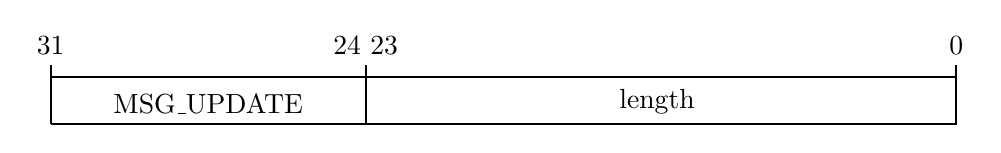
\begin{tikzpicture}
\draw[thick] (0,0) -- (11.5,0) -- (11.5,0.6) -- (0,0.6) -- (0,0);
\draw[thick] (0,0) -- (0,0.75) node[above] {31};
\draw[thick] (4,0) -- (4,0.75) node[above] {24 23};
\draw[thick] (11.5,0) -- (11.5,0.75) node[above] {0};
\draw[thick] (2,0) node[above] {MSG\_UPDATE};
\draw[thick] (7.7,0.00) node[above] {length};
\end{tikzpicture}

\bigskip

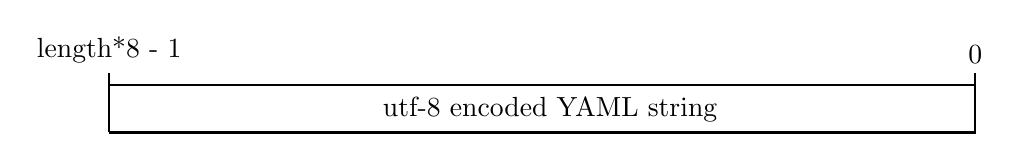
\begin{tikzpicture}
\draw[thick] (0,0) -- (11,0) -- (11,0.6) -- (0,0.6) -- (0,0);
\draw[thick] (0,0) -- (0,0.75) node[above] {length*8 - 1};
\draw[thick] (11,0) -- (11,0.75) node[above] {0};
\draw[thick] (5.6,0) node[above] {utf-8 encoded YAML string};
\end{tikzpicture}
\end{minipage}

\subsubsection{MENU NUM ITEMS}
\label{server_menu_num_items}
\hfill\begin{minipage}{\dimexpr\textwidth-1.4cm}
In response to a MENU REQUEST (section \ref{menureq} on page \pageref{menureq}),
a server should send a single instance of the following 16-bit (2-byte) packet:

\vspace{0.2cm}

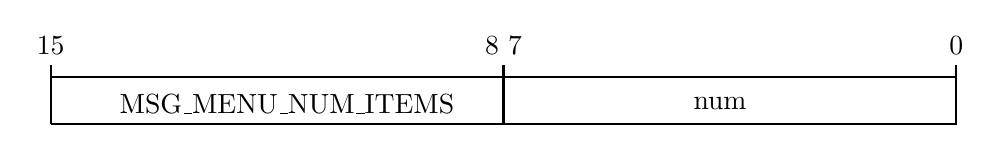
\begin{tikzpicture}
\draw[thick] (0,0) -- (11.5,0) -- (11.5,0.6) -- (0,0.6) -- (0,0);
\draw[thick] (0,0) -- (0,0.75) node[above] {15};
\draw[thick] (5.75,0) -- (5.75,0.75) node[above] {8 7};
\draw[thick] (11.5,0) -- (11.5,0.75) node[above] {0};
\draw[thick] (3,0) node[above] {MSG\_MENU\_NUM\_ITEMS};
\draw[thick] (8.5,0.05) node[above] {num};
\end{tikzpicture}

\vspace{0.5cm}

The ''num'' field should contain the number of MENU ITEMs
(section \ref{server_menu_item} on page \pageref{server_menu_item})
that will follow. After sending this packet a server should
immediately send ''num'' number of MENU ITEMs.
\end{minipage}

\vspace{0.5cm}

\subsubsection{MENU ITEM}
\label{server_menu_item}
\hfill\begin{minipage}{\dimexpr\textwidth-1.4cm}
To define an action that a client is allowed to perform at
the current time (immediately after receiving the message),
a server should send the following 40-bit (5-byte) packet:

\vspace{0.2cm}

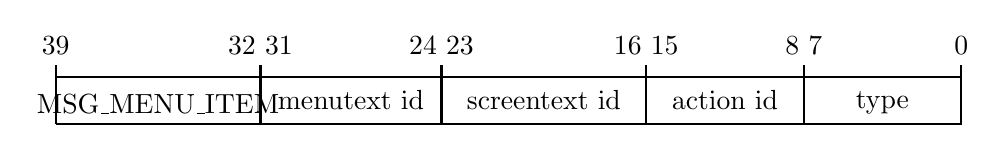
\begin{tikzpicture}
\draw[thick] (0,0) -- (11.5,0) -- (11.5,0.6) -- (0,0.6) -- (0,0);
\draw[thick] (0,0) -- (0,0.75) node[above] {39};
\draw[thick] (2.6,0) -- (2.6,0.75) node[above] {32 31};
\draw[thick] (4.9,0) -- (4.9,0.75) node[above] {24 23};
\draw[thick] (7.5,0) -- (7.5,0.75) node[above] {16 15};
\draw[thick] (9.5,0) -- (9.5,0.75) node[above] {8 7};
\draw[thick] (11.5,0) -- (11.5,0.75) node[above] {0};
\draw[thick] (1.3,0) node[above] {MSG\_MENU\_ITEM};
\draw[thick] (3.75,0.06) node[above] {menutext id};
\draw[thick] (6.2,0.06) node[above] {screentext id};
\draw[thick] (8.5,0.06) node[above] {action id};
\draw[thick] (10.5,0) node[above] {type};
\end{tikzpicture}

\vspace{0.5cm}

The ''menutext id'' field should contain the numeric key of the
string contained in the language dataset that a client should
display in the user interface where the user is supposed
to select the action (before the action has been selected).

\vspace{0.3cm}

The ''screentext id'' field should contain the numeric key of
the string contained in the language dataset that a client should
display to the user when the user has selected to perform the action
(after the action has been selected).

\vspace{0.3cm}

The ''action id'' field should contain an ID that the server
wishes to receive as part of the ACTION (section \ref{action} on page \pageref{action})
sent by a client executing the action.

\vspace{0.3cm}

The ''type'' field is used for bitwise flags as specified by the
symbolic constants prefixed with TYPE\_ (section \ref{constants} on page \pageref{constants}).

\vspace{0.3cm}

Including the flag of TYPE\_SND\_UINT32 instructs clients to read
input from the user and to include the value of said input in the
''param'' field of the ACTION.

\vspace{0.3cm}

Including the flag of TYPE\_RECV\_UINT32 instructs clients to receive
a RESPONSE (section \ref{server_response} on page \pageref{server_response})
from the server directly after having sent an ACTION. If this flag is
not included, clients are instead instructed to receive an OK
(section \ref{server_ok} on page \pageref{server_ok})or a FAIL
(section \ref{server_fail} on page \pageref{server_fail}) directly
after sending the ACTION. The server must send the appropriate
response (RESPONSE, OK or FAIL) directly after having received
the ACTION.

\end{minipage}

\hfill\begin{minipage}{\dimexpr\textwidth-1.4cm}

Including the flag of TYPE\_RECV\_FOLLOWUP instructs clients to
receive a MENU ITEM (section \ref{server_menu_item} on page \pageref{server_menu_item})
after having sent the ACTION and having read the response (RESPONSE,
OK or FAIL) described in the previous paragraph. This MENU ITEM instructs
a client to perform another ACTION immediately following the previous
one. Any number of these exchanges can be chained together. A server
that sends a MENU ITEM including this flag must send the follow-up
MENU ITEM directly after having sent the initial response to the
ACTION (RESPONSE, OK or FAIL) as described in the previous paragraph.


\end{minipage}

\subsubsection{RESPONSE}
\label{server_response}
\hfill\begin{minipage}{\dimexpr\textwidth-1.4cm}
To respond to an ACTION (section \ref{action} on page \pageref{action})
with type TYPE\_RECV\_UINT32, a server should send the following
56-bit (7-byte) packet:

\vspace{0.2cm}

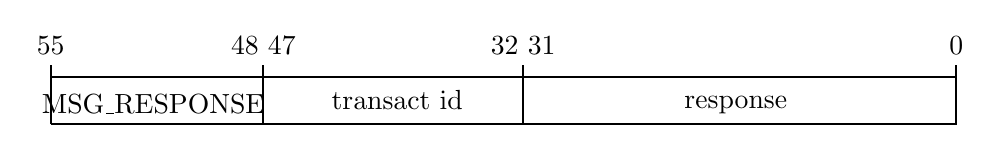
\begin{tikzpicture}
\draw[thick] (0,0) -- (11.5,0) -- (11.5,0.6) -- (0,0.6) -- (0,0);
\draw[thick] (0,0) -- (0,0.75) node[above] {55};
\draw[thick] (2.7,0) -- (2.7,0.75) node[above] {48 47};
\draw[thick] (6,0) -- (6,0.75) node[above] {32 31};
\draw[thick] (11.5,0) -- (11.5,0.75) node[above] {0};
\draw[thick] (1.3,0) node[above] {MSG\_RESPONSE};
\draw[thick] (4.4,0.06) node[above] {transact id};
\draw[thick] (8.7,0) node[above] {response};
\end{tikzpicture}

\vspace{0.5cm}

The ''transact id'' field should contain the exact value received in
the ''transact id'' field of the ACTION that is being responded to.

\vspace{0.3cm}

The ''response'' field should contain a numeric response to the
ACTION, suitable for a client to display for a user.
\end{minipage}

\subsubsection{OK}
\label{server_ok}
\hfill\begin{minipage}{\dimexpr\textwidth-1.4cm}
To respond to a successfully performed ACTION (section \ref{action} on page \pageref{action})
that was not flagged with type TYPE\_RECV\_UINT32, a server should send the following
24-bit (3-byte) packet:

\vspace{0.2cm}

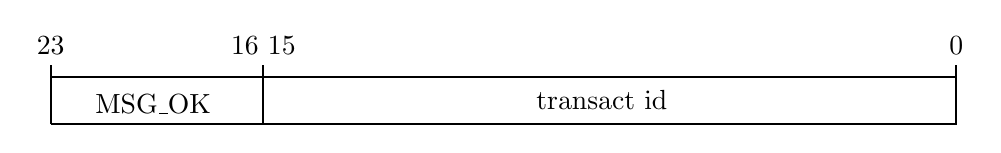
\begin{tikzpicture}
\draw[thick] (0,0) -- (11.5,0) -- (11.5,0.6) -- (0,0.6) -- (0,0);
\draw[thick] (0,0) -- (0,0.75) node[above] {23};
\draw[thick] (2.7,0) -- (2.7,0.75) node[above] {16 15};
\draw[thick] (11.5,0) -- (11.5,0.75) node[above] {0};
\draw[thick] (1.3,0) node[above] {MSG\_OK};
\draw[thick] (7,0.06) node[above] {transact id};
\end{tikzpicture}

\vspace{0.5cm}

The ''transact id'' field should contain the exact value received in
the ''transact id'' field of the ACTION that is being responded to.

\end{minipage}

\subsubsection{FAIL}
\label{server_fail}
\hfill\begin{minipage}{\dimexpr\textwidth-1.4cm}
To respond to a failed ACTION (section \ref{action} on page \pageref{action})
that was not flagged with type TYPE\_RECV\_UINT32, a server should send the following
32-bit (4-byte) packet:

\vspace{0.2cm}

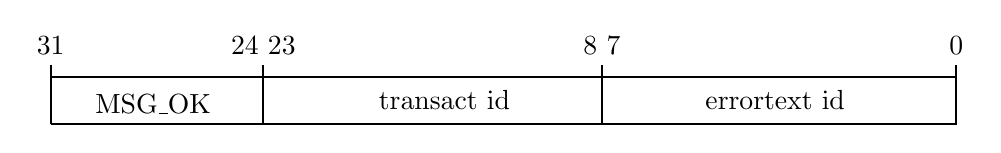
\begin{tikzpicture}
\draw[thick] (0,0) -- (11.5,0) -- (11.5,0.6) -- (0,0.6) -- (0,0);
\draw[thick] (0,0) -- (0,0.75) node[above] {31};
\draw[thick] (2.7,0) -- (2.7,0.75) node[above] {24 23};
\draw[thick] (7,0) -- (7,0.75) node[above] {8 7};
\draw[thick] (11.5,0) -- (11.5,0.75) node[above] {0};
\draw[thick] (1.3,0) node[above] {MSG\_OK};
\draw[thick] (5,0.06) node[above] {transact id};
\draw[thick] (9.2,0.06) node[above] {errortext id};
\end{tikzpicture}

\vspace{0.5cm}

The ''transact id'' field should contain the exact value received in
the ''transact id'' field of the ACTION that is being responded to.

\vspace{0.3cm}

The ''errortext id'' field should contain the numeric key of a
string contained in the language dataset that explains the nature
of the failure suitable for a client to display to a user.
\end{minipage}

\newpage
\section{EXAMPLE SESSIONS}

\bigskip
The following example session is illustrating a session where everything is 
going great.

\begin{figure}[H]
\centering
\includegraphics[scale=0.8]{Session_ok.png}
\caption{Example session 1}
\end{figure}

\bigskip
This example session is illustrating a session where
an error occurs.

\begin{figure}[H]
\centering
\includegraphics[scale=0.8]{Session_fail.png}
\caption{Example session 2}
\end{figure}

\end{document}
